\chapter{Návrh ovládacích karet}
\section{Základní požadavky na Ovládací karty}
    Následující seznam popisuje základní požadavky na ovládací karty, seznam je seřazen podle priorit.
    Obdobně jako v kapitole o měřících kartách jsou schémata i v této kapitole ilustrační a přesné zapojení
    lze nalézt v příloze. 
    \begin{enumerate}
        \item Schopnost ovládat měřící karty.
        \item Možnost komunikace pomocí 100\,Mbit Ethernetu a USB.
        \item Dostupnost komponentů.
        \item Cena komponentů.
    \end{enumerate}

    \section{Funkční bloky}
    \begin{figure}[ht!]
        \centering
        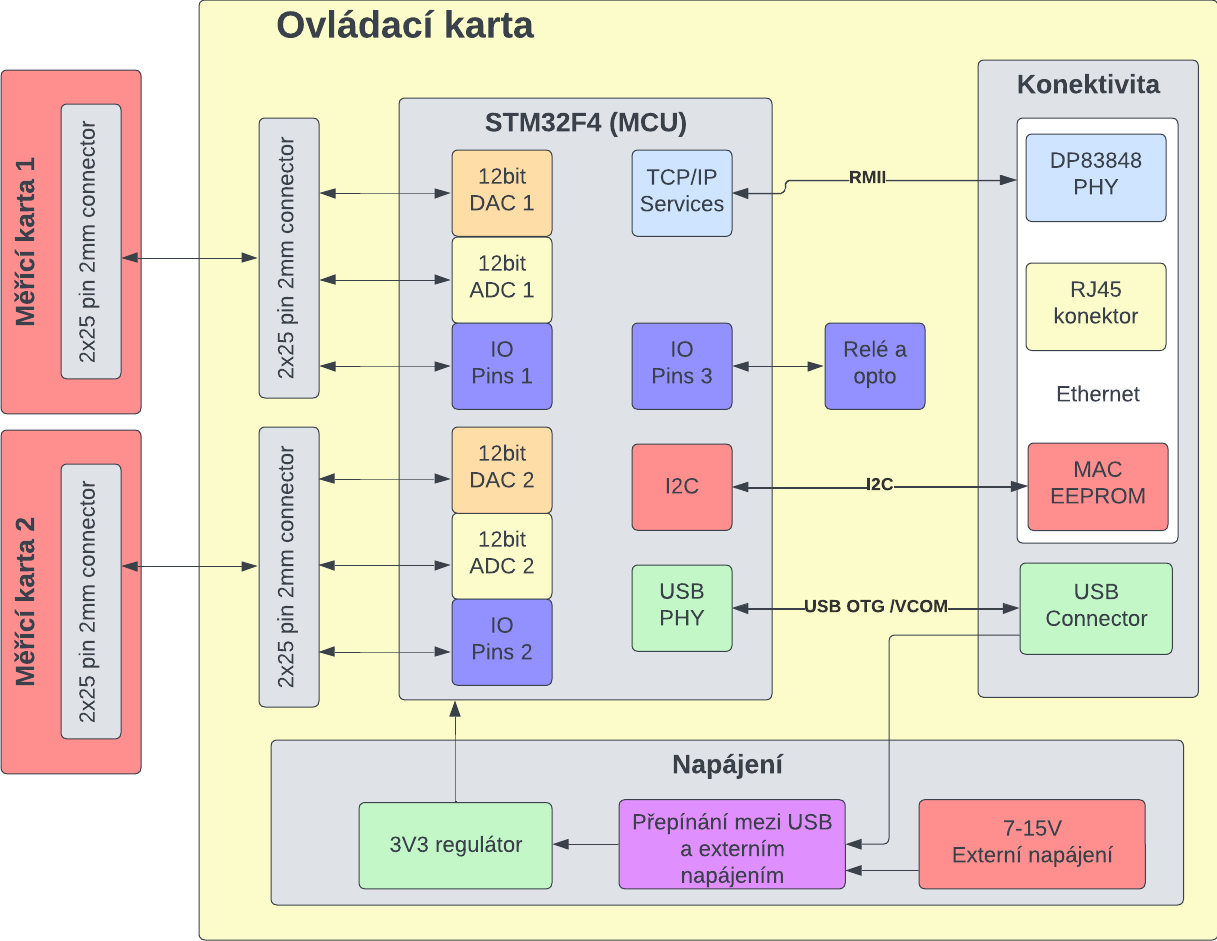
\includegraphics[width = 1\textwidth]{obrazky/ovladaci_karta_diag.png}
        \caption{Funkční diagram ovládací karty}
        \label{fig:Funkční diagram ovládací karty}
        
    \end{figure}

    Ovládací karta obsahuje několik pomyslných funkčních bloků (Obr. \ref{fig:Funkční diagram ovládací karty}).
    Jednotlivé bloky jsou podrobněji popsány v následujících kapitolách. Celé schéma k ovládací kartě je v příloze
    na konci tohoto dokumentu.

    \subsection{Mikrokontrolér a jeho periférie}
    Ovládací karta je založena na 32bitovém
    mikrokontroléru STM32F407ZGT6 s Cortex M4 jádrem.
    Tento mikrokontrolér disponuje 114 I/O piny (3V3 logika), dvěma nezávislými 12bitovými A/D a D/A převodníky,
    nativní podporou USB OTG a 100\,Mbit Ethernet MAC vrstvou. Právě díky těmto vlastnostem, je tento
    mikrokontrolér vhodný pro ovládání měřících karet a komunikaci s PC.\par

    Pro komunikaci s PC aplikací se primárně počítá s telnet serverem,
    který běží na mikrokontroléru. Nicméně pro ladící (debugovací)
    účely je možno s ovládací kartou komunikovat i pomocí USB.
    K programování mikrokontroléru lze použít rozhraní SWD, JTAG nebo DFU (USB bootloader)\cite{MARTINT}.\par

    Jednotlivé shift registry a multiplexery měřící karty jsou ovládány, skrze ovládací kartu, pomocí metody bit bangingu.
    Ovládací karta obsahuje i další periferie jako například CAN, LIN, RTC, opticky oddělené vstupy a výstupy apod.
    Tyto periferie slouží k použití karty v jiném projektu, který není obsahem diplomová práce, a proto nejsou podrobněji diskutovány.


    \subsubsection{D/A převodník}
    STM32F407ZGT6 nabízí dva 12bitové D/A převodníky s možností využití integrovaného bufferu v podobě
    invertujícího operačního zesilovače. Nicméně podle datasheetu
    je možné použít výstupní buffer pouze do velikosti kapacitní zátěže 50\,pF.
    Kapacitní zátěž D/A převodníku bude rovna parazitním kapacitám, které nelze jednoznačně určit
    a vstupní kapacitě 80 komparátorů (V+ proti GND). Každý z komparátorů má svou vstupní kapacitu
    přibližně 3\,pF. Dohromady tedy vznikne kapacitní zátěž minimálně 240\,pF.\cite{DAC}\par

    \begin{figure}[ht!]
        \centering
        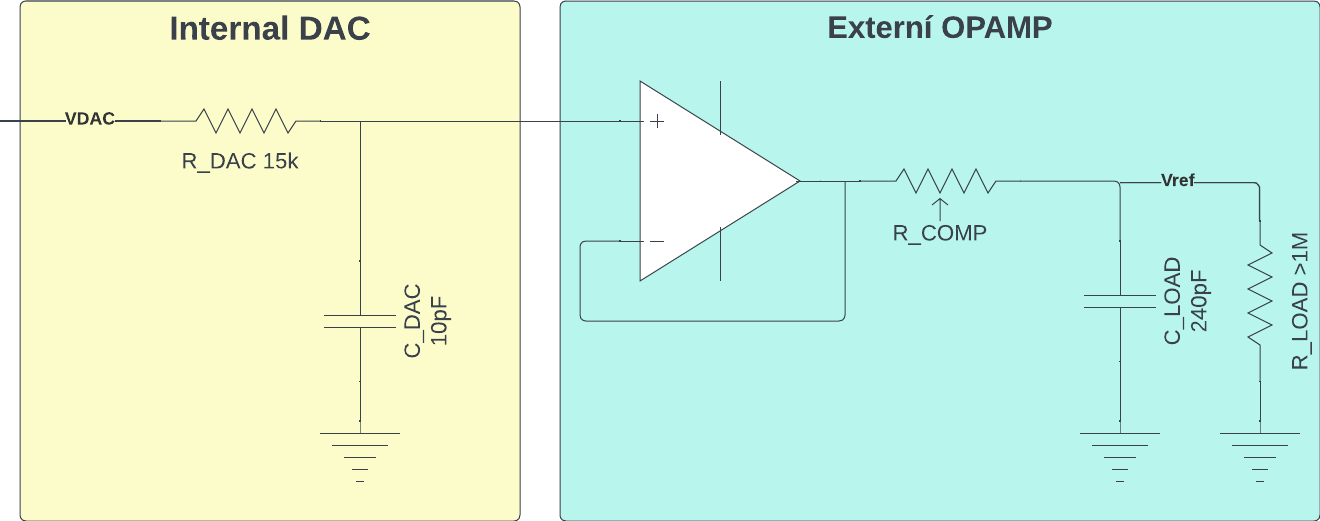
\includegraphics[width = 1\textwidth]{obrazky/DAC_OPAMP.png}
        \caption{DAC-externí zesilovač}
        \label{fig: DAC-externí zesilovač}
        
    \end{figure}

    Pro použití D/A převodníku je použit externí operační zesilovač v zapojení (Obr. \ref{fig: DAC-externí zesilovač}).
    V tomto zapojení je rychlost D/A převodníku limitována kapacitou pinu D/A převodníku C\_DAC (cca 10\,pF)
    a vnitřním odporem R\_DAC (cca 15\,k$\Omega$). Mezní kmitočet nezatíženého D/A převodníku pak lze určit následovně.
    \begin{equation}
        f_{max} = \frac{1}{2\pi \cdot  C_{dac} \cdot  R_{dac}} = \frac{1}{2\pi \cdot 10\,pF \cdot 15\,k\Omega} = 1,06\,MHz
    \end{equation}

    Kapacitní zátěž společně s výstupním odporem operačního zesilovače by mohla
    způsobit nestabilitu a s tím spojené nežádoucí oscilace v časové oblasti.
    Z tohoto důvodu datasheet použitého operačního zesilovače AD8531 doporučuje použít v případě vyšší kapacitní zátěže tzv. snubber network.
    V datasheetu je možno nalézt následující hodnoty součástek pro různou kapacitní zátěž (v Obr. \ref{fig: DAC-externí zesilovač} realizováno
    kombinací součástek C\_SNUBB a R\_COMP).

    \begin{table}[ht!]
        \centering
        \begin{tabular}{|l|l|l|}
        \hline
        \textbf{Load Capacitance (CL)} & \textbf{Rs{[}Ohm{]}} & \textbf{Cs {[}uF{]}} \\ \hline
        \textbf{0.47nF}                & 300                  & 0.1                  \\ \hline
        \textbf{4.7nF}                 & 30                   & 1                    \\ \hline
        \textbf{47nF}                  & 5                    & 1                    \\ \hline
        \textbf{240pF (zvolené hodnoty)}                  &100$\Omega$ Trimmer        & 0.1                      \\ \hline
        \end{tabular}%

        \caption{Snubber Network (Přepis tabulky z datasheetu \cite{OPA_datasheet})}
        \label{tab:SnubberNetwork}
    \end{table}

    Protože datasheet neuvádí hodnoty součástek pro kapacitní zátěž 240\,pF, je odpor R\_COMP realizován
    trimmerem pro možnost kalibrace. Hodnota kapacity C\_SNUBB byla zvolena 100\,nF.\par

    Kalibrace je prováděna tak, že se na výstupu D/A převodníku nastaví obdélníkový
    signál o frekvenci 500\,kHz a poté se trimmerem nastaví taková hodnota, aby v časové oblasti
    byl co nejmenší překmit\cite{DAC_stability,OPA_stability}.\par

    \subsubsection{Programování a debuging}
    Pro účely debugování a programování mikrokontroléru jsou zpřístupněny SWD a JTAG piny.
    Dále je možno modifikovat konfiguraci mikrokontroléru pomocí jumperů, které jsou propojeny
    s boot piny mikrokontroléru. Při normálním provozu se počítá s programováním pomocí SWD rozhraní.
    Případně je také možné mikrokontrolér naprogramovat přes USB konektor pomocí zabudovaného DFU.

    \subsubsection{Konfigurace hodinového signálu}
    
    Mikrokontrolér má vysokou variabilitu v konfiguraci hodinových signálů.
    K požadovaným funkcím ovládací karty je vhodné použít externí krystalový rezonátor, který bude
    připojen do High Speed Clock pinů mikrokontroléru. V případě ovládací karty bylo použit 8\,MHz
    krystalového rezonátoru ABM3B-8.000MHZ-D2-T společně s 2x27\,pF zatěžovacími kapacitory.\par

    %%\begin{figure}[ht!]
    %%    \centering
    %%    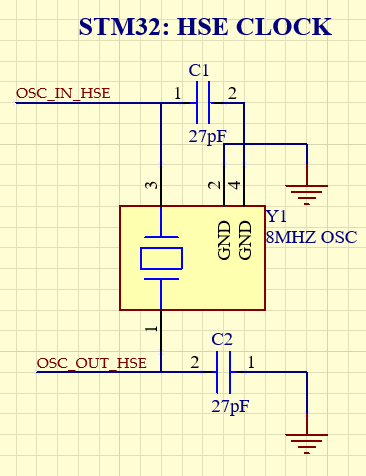
\includegraphics[height = 0.2\textheight]{obrazky/CLK_rezonator.png}
    %%    \caption{8\,MHz krystalový rezonátor}
    %%    \label{fig: MHz krystalový rezonátor}
    %%\end{figure}

    Pro jednodušší konfiguraci hodinových signálů mikrokontroléru bylo využito programu STM32CubeMX.
    Výsledná konfigurace hodinových signálů je znázorněna na následujícím obrázku.
    \begin{figure}[ht!]
        \centering
        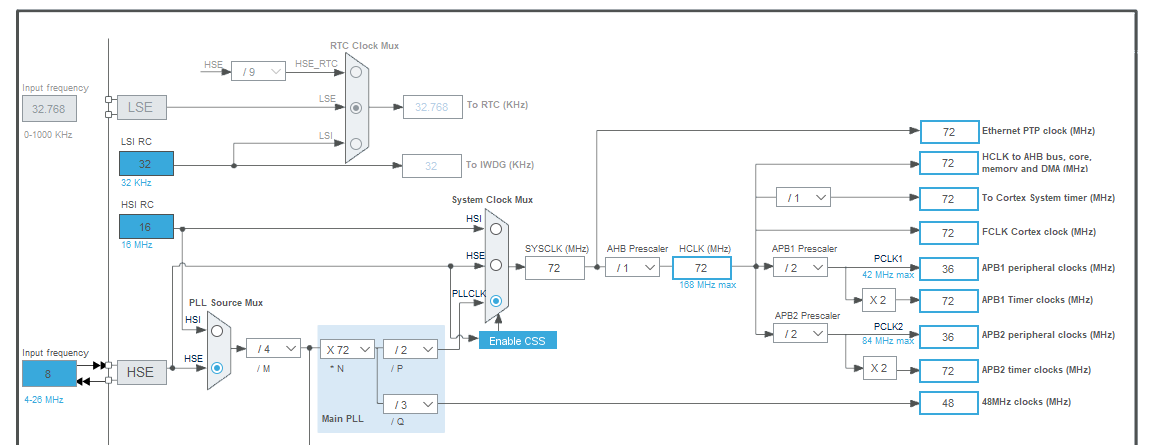
\includegraphics[width = 1\textwidth]{obrazky/CLK_config.png}
        \caption{Konfigurace hodinových signálů - STM32CubeMX}
        \label{fig: Clock configuration}
    \end{figure}

    \subsection{Konektivita}
    Ovládací karta je vybavena USB-micro a RJ45 konektorem. Umožňuje tak velmi snadné propojení s PC aplikací
    pomocí standardních USB a ethernetových rozhraní.

    \subsubsection{Ethernet}
    Pro zajištění ethernetového připojení je využito MAC
    vrstvy mikrokontroléru společně s fyzickou vrstvou (PHY)
    realizovanou pomocí čipu DP83848 a RJ45 konektoru s integrovaným transformátorem pro 100 BASE-T. Komunikace mezi
    mikrokontrolérem a DP83848 je realizováno pomocí RMII rozhraní. PHY vyžaduje pro svou správnou funkčnost
    100$\Omega$ diferenciální páry (viz. schéma ovládací karty v příloze).\par
    
    DP83848 vyžaduje pro svou činnost v RMII režimu připojení externího 50\,MHz oscilátoru.
    Výstup oscilátoru je zároveň přiveden na příslušný pin mikrokontroléru a slouží jako 
    hodinová reference.\par

    DP83848 je možno konfigurovat pomocí tzv. bootstrap pinů. DP83848 při svém startu zjišťuje
    logické úrovně bootstrap pinů a podle toho konfiguruje své parametry. Následující tabulka
    shrnuje nastavení bootstrap pinů použitých v ovládací kartě.

    \begin{table}[ht!]
        \resizebox{\columnwidth}{!}{%
        \begin{tabular}{|c|c|l|}
        \hline
        \textbf{PIN} & \textbf{Nastavení} & \textbf{Popis}                                   \\ \hline
        AN0 & 1 & AN0 a AN1 piny konfigurují, jakými možnostmi se bude zařízení prezentovat   při AutoNegotioation.   \\ \hline
        AN1 & 1 & Pro kombinaci AN0 = 1 a AN1 = 1 zařízení se prezentuje jako  10BASE-T a 100BASE-TX HALF/FULL duplex \\ \hline
        LED\_CFG     & 1                  & Konfiguruje chování LED na RJ45 konektoru.       \\ \hline
        MII\_MODE    & 1                  & DP83848 očekává RMII pro komunikaci s MAC vrstvou \\ \hline
        MDIX ENABLE  & 1                  & Interní pull up - MDIX (crossover) povolen       \\ \hline
        \end{tabular}%
        }
        \caption{Nastavení bootstrap pinů DP83848}
        \label{RMII settings}
        \end{table}


    Protože ani mikrokontrolér a ani DP83848 nenabízí jedinečnou MAC adresu je použita EEPROM,
    která má již od výrobce naprogramovanou jedinečnou MAC adresu.
    EEPROM používá ke komunikaci I2C protokol a při startu zařízení je MAC adresa
    načtena do MAC vrstvy mikrokontroléru. V mikrokontroléru je implementován telnet
    a http server a je využito LWIP stacku společně s HAL knihovnami a Free-RTOS.\par

    \subsubsection{USB}
    Mikrokontrolér je vybaven fyzickou vrstvou pro USB OTG,
    je tak možné propojit datové signály přímo s USB-micro konektorem.
    Přestože je do USB konektoru vyveden ID pin, který slouží
    k rozlišení zařízení mezi host a device, využívá ovládací karta pouze režim device.
    Pro detekci připojení ovládací karty k USB portu je použit napěťový dělič, jehož výstup
    je přiveden do USB\_sense pinu mikrokontroléru. Napěťový dělič obsahuje rezistor o toleranci
    1\,\%. Tuto toleranci není nutno dodržet a tento rezistor byl použit pouze z důvodu nízké ceny
    a faktu, že se již v návrhu vyskytuje.\par

    Připojení pomocí USB slouží převážně k servisním účelům.
    Ovládací kartu lze napájet přímo z USB portu, přičemž napájení je opatřeno
    vstupním filtrem realizovaným feritovou perličkou a kondenzátorem (více v sekci o napájení).
    Obdobně jako u ethernetu je i zde nutno při návrhu PCB použít diferenciální páry
    pro datové signály (90\,$\Omega$). Každý ze signálů,
    který je vyveden na USB-micro konektor je opatřen TVS diodami pro ochranu
    proti ESD.\par

    \begin{figure}[ht!]
        \centering
        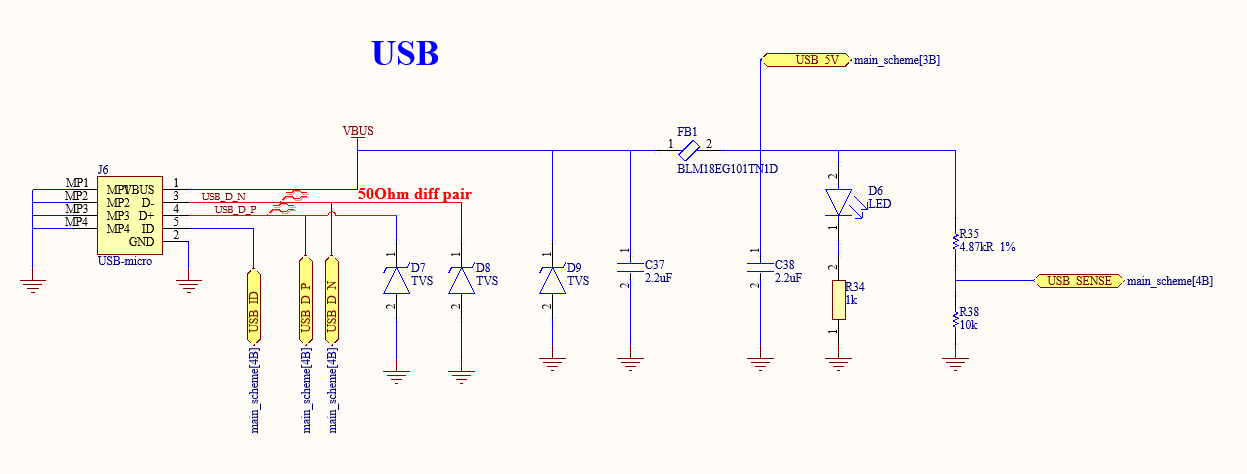
\includegraphics[width = 1\textwidth]{obrazky/USB.png}
        \caption{USB rozhraní}
        \label{fig: USB rozhraní}
    \end{figure}

\clearpage
    \subsection{Napájení}
    Při normálním provozu se počítá s externím napájení v rozmezí 7-9 VDC.
    Toto napětí je přivedeno na WAGO svorky. Napětí (ve schématu BOARD\_PWR)
    přivedeno na vstup nastavitelného regulátoru TLV76701DGNR. Funkce tohoto regulátoru je obdobná
    jako u regulátorů popsaných v sekci o měřící kartě. Výstup regulátoru je možné
    nastavit trimmerem v rozmezí přibližně od 2.8 do 3.45V (ve schématu 3v3\_MCUs).\par

    \begin{figure}[ht!]
        \centering
        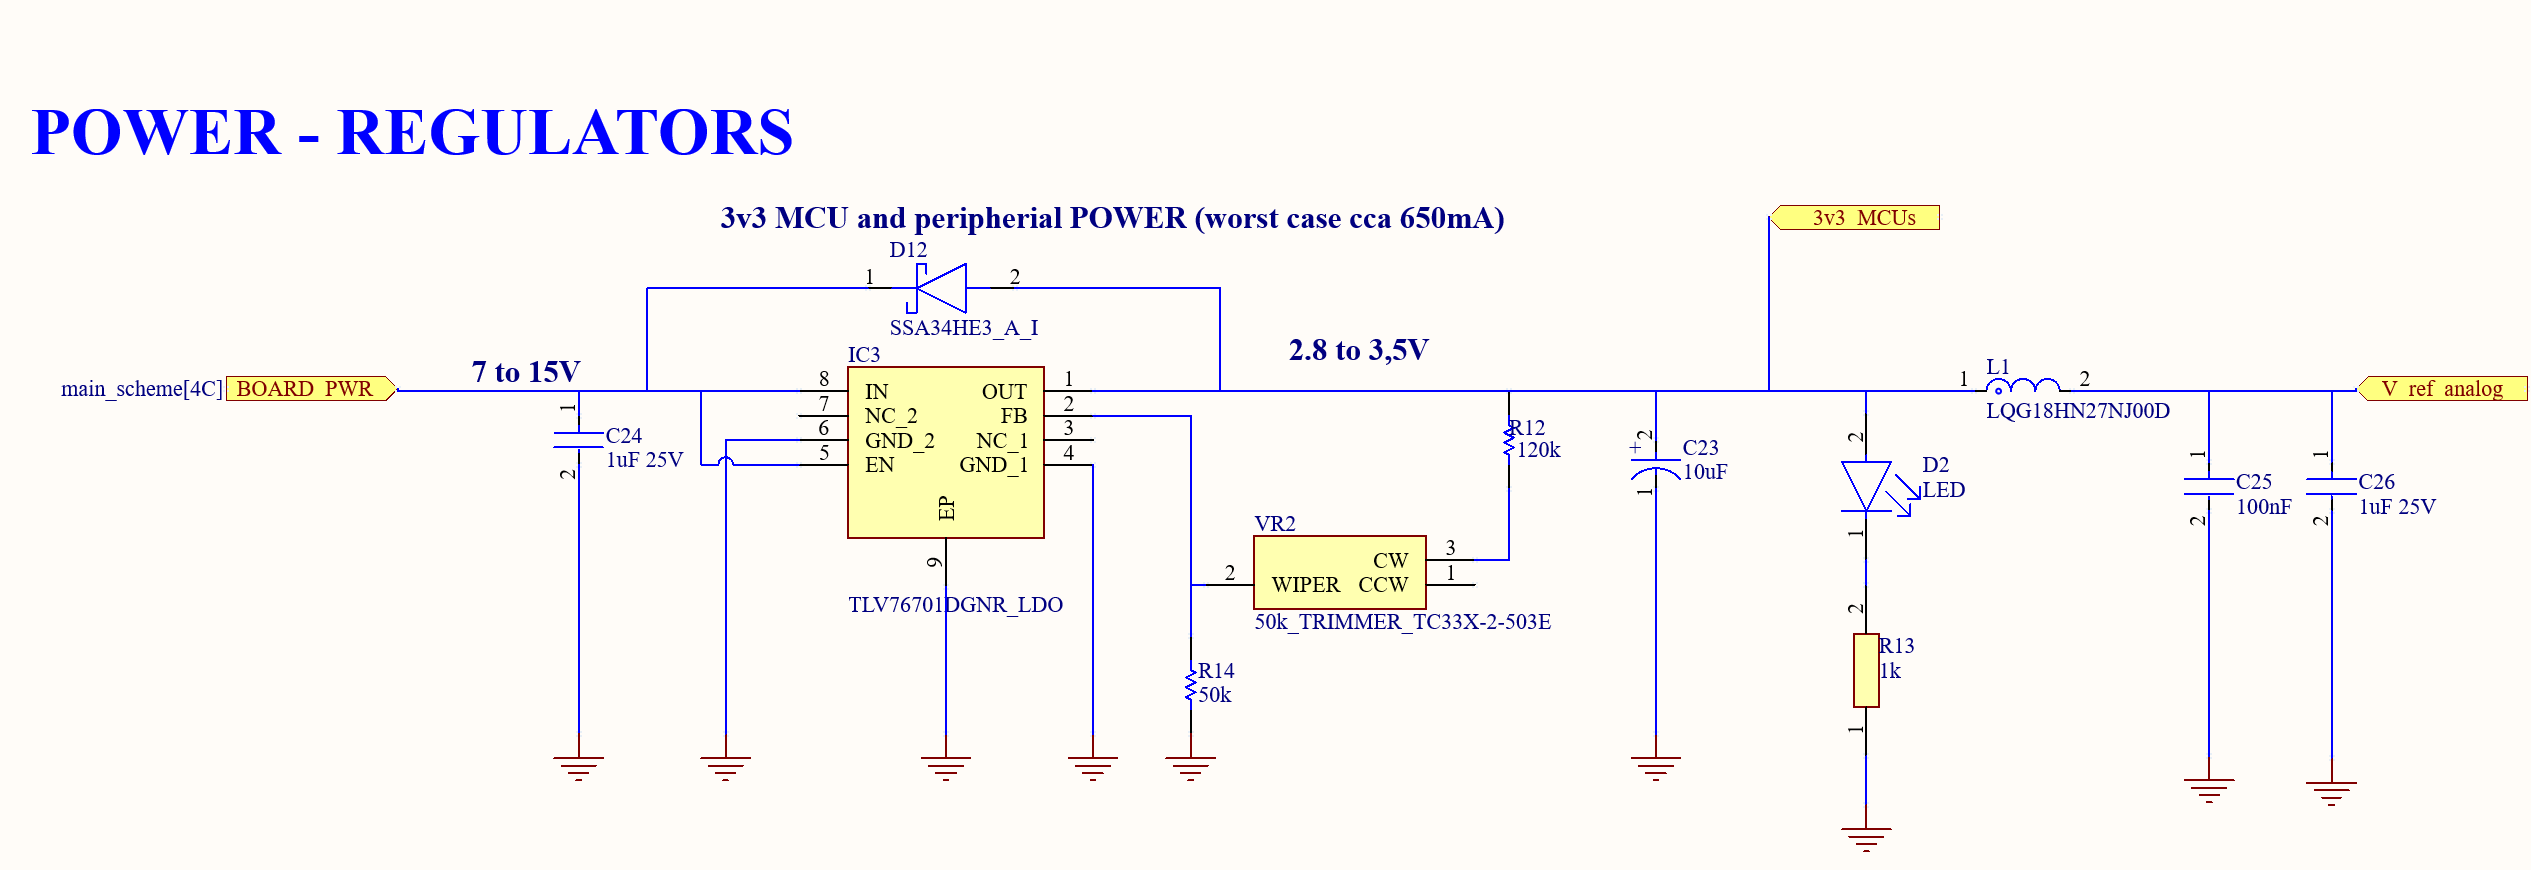
\includegraphics[width = 1\textwidth]{obrazky/PWR_REG_3V3.png}
        \caption{Regulátor napětí - 3V3 MCUs}
        \label{fig:Regulátor napětí - 3V3 MCUs}
    \end{figure}

    Takto regulované napětí je použito pro napájení všech doposud popsaných částí ovládací karty.
    Protože je vhodné, aby referenční napětí (V\_ref\_analog),
    které mikrokontrolér používá  pro funkci A/D a D/A převodníků bylo co nejpřesnější, je
    napětí 3V3\_MCUs filtrováno dolní propustí realizovanou pomocí LC filtru.\par

    Očekávaný maximální proud fyzické vrstvy ethernetu je přibližně 150\,mA.
    Proudový odběr ovládací karty nelze jednoznačně určit,
    protože je závislý na firmwaru mikrokontroléru.
    Nicméně se očekává, že by proud tímto regulátorem v nejhorším případě neměl přesáhnout 400\,mA. 
    Použitý regulátor by měl být schopen dodat do obvodu proud přibližně 450\,mA (viz. \ref{section: REGULATOR_POWER}).
    
    Napětí je dále přivedeno na 2x25pinový konektor,
    aby bylo možné napájet měřící a ovládací karty současně připojením napájecí napětí pouze
    na jednu z karet.\par

    Celý systém měřících a ovládacích karet může být napájen pomocí USB. V tomto případě je však přesnost
    měření limitována kvalitou USB napájení. Následující obrázek znázorňuje distribuci napájení
    ovládacích a měřících karet. Schéma však neodpovídá reálnému zapojení, protože jednotlivé
    komponenty jsou propojeny přes 2x25 pin konektory. Pro přehlednost jsou však konektory vynechány.
    \clearpage


    \begin{figure}[ht!]
        \centering
        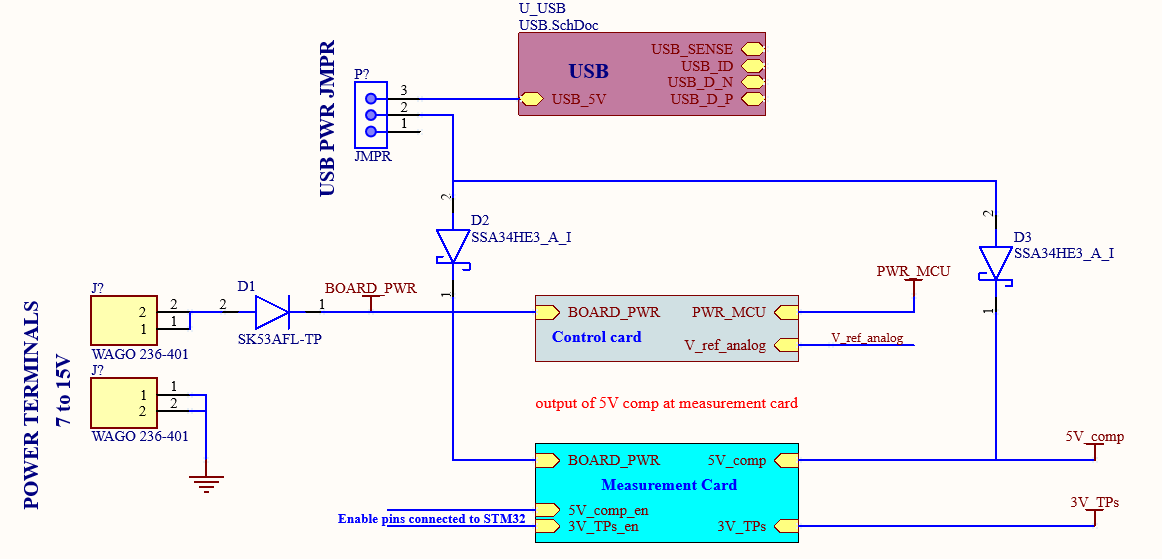
\includegraphics[width = 1\textwidth]{obrazky/USB_power_distr.png}
        \caption{Distribuce napájení}
        \label{fig:Distribuce napájení}
    \end{figure}

    V případě napájení pomocí USB je napětí BOARD\_PWR generováno z USB portu.
    Aby se zamezilo poškození všech připojených zařízení, které by mohlo potenciálně vzniknout připojením
    vyššího napětí na WAGO svorkách a USB současně, je do schématu připojena dioda D2. Dioda D1
    slouží jako ochrana k přepólování na vstupu WAGO svorek. Zároveň dioda D1 plní obdobnou funkci jako dioda D2
    nyní však pro ochranu zdroje napájení připojeného do WAGO svorek proti napětí na USB.
    V případě současného připojení externího napětí na WAGO svorky a USB portu, bude deska napájena
    vyšším z napětích.
    Napětí BOARD\_PWR je v případě napájení přes USB rovno přibližně:
    \begin{equation}
        V_{BOARD\_PWR} = V_{USB} - V_{D2} = 5V - 0.4V = 4.6V,
    \end{equation}
    kde $V_{D2}$ je úbytek na diodě D2. Tento úbytek je pro diodu SSA34HE3\_A\_I roven přibližně 0.2V při proudu 1A
    a přibližně 0.4V při proudu 2A\par

    Úbytek napětí na regulátorech TLV76701DGNR je přibližně 0.8V.
    Součtem úbytků na diodě D2 a regulátoru lze 
    dosáhnou regulovaného výstupního napětí až 3.8V, což je dostatečné pro napájení všech regulátorů
    kromě regulátoru, který zajišťuje napětí 5V\_comp. Napětí 5V\_comp je tedy generováno přímo z USB portu přes 
    diodu D3. Dioda D3 má obdobný význam jako dioda D2, nyní však chrání USB port před vyšším napětím na výstupu
    regulátoru 5V\_comp v případě napájení z WAGO svorek. Z tohoto je patrné, že napětí 5V\_comp není nijak regulováno
    a je přímo závislé na napětí a rušení USB portu.
    V případě detekce napětí na USB\_sense pinu je komparátor 5V\_comp vypnut pomocí enable pinu.\par

    Pro možnost použití USB rozhraní pouze pro komunikaci (ne pro napájení),
    lze USB napájení rozpojit pomocí zkratovací propojky.\par
\clearpage

\subsection{PCB design}
   Stejně jako u návrhu měřící karty byl při návrhu ovládací karty použit software ALTIUM Designer.
   PCB je 6vrstvé s řízenými impedancemi pro diferenciální páry USB a Ethernet fyzických vrstev.
   Pro určité cesty je zajištěna stejná délka cest pro správnou funkčnost rychlých signálů.
   Podrobnější informace lze nalézt v příloze diplomové práce.\par
\begin{figure}[ht!]
    \centering
    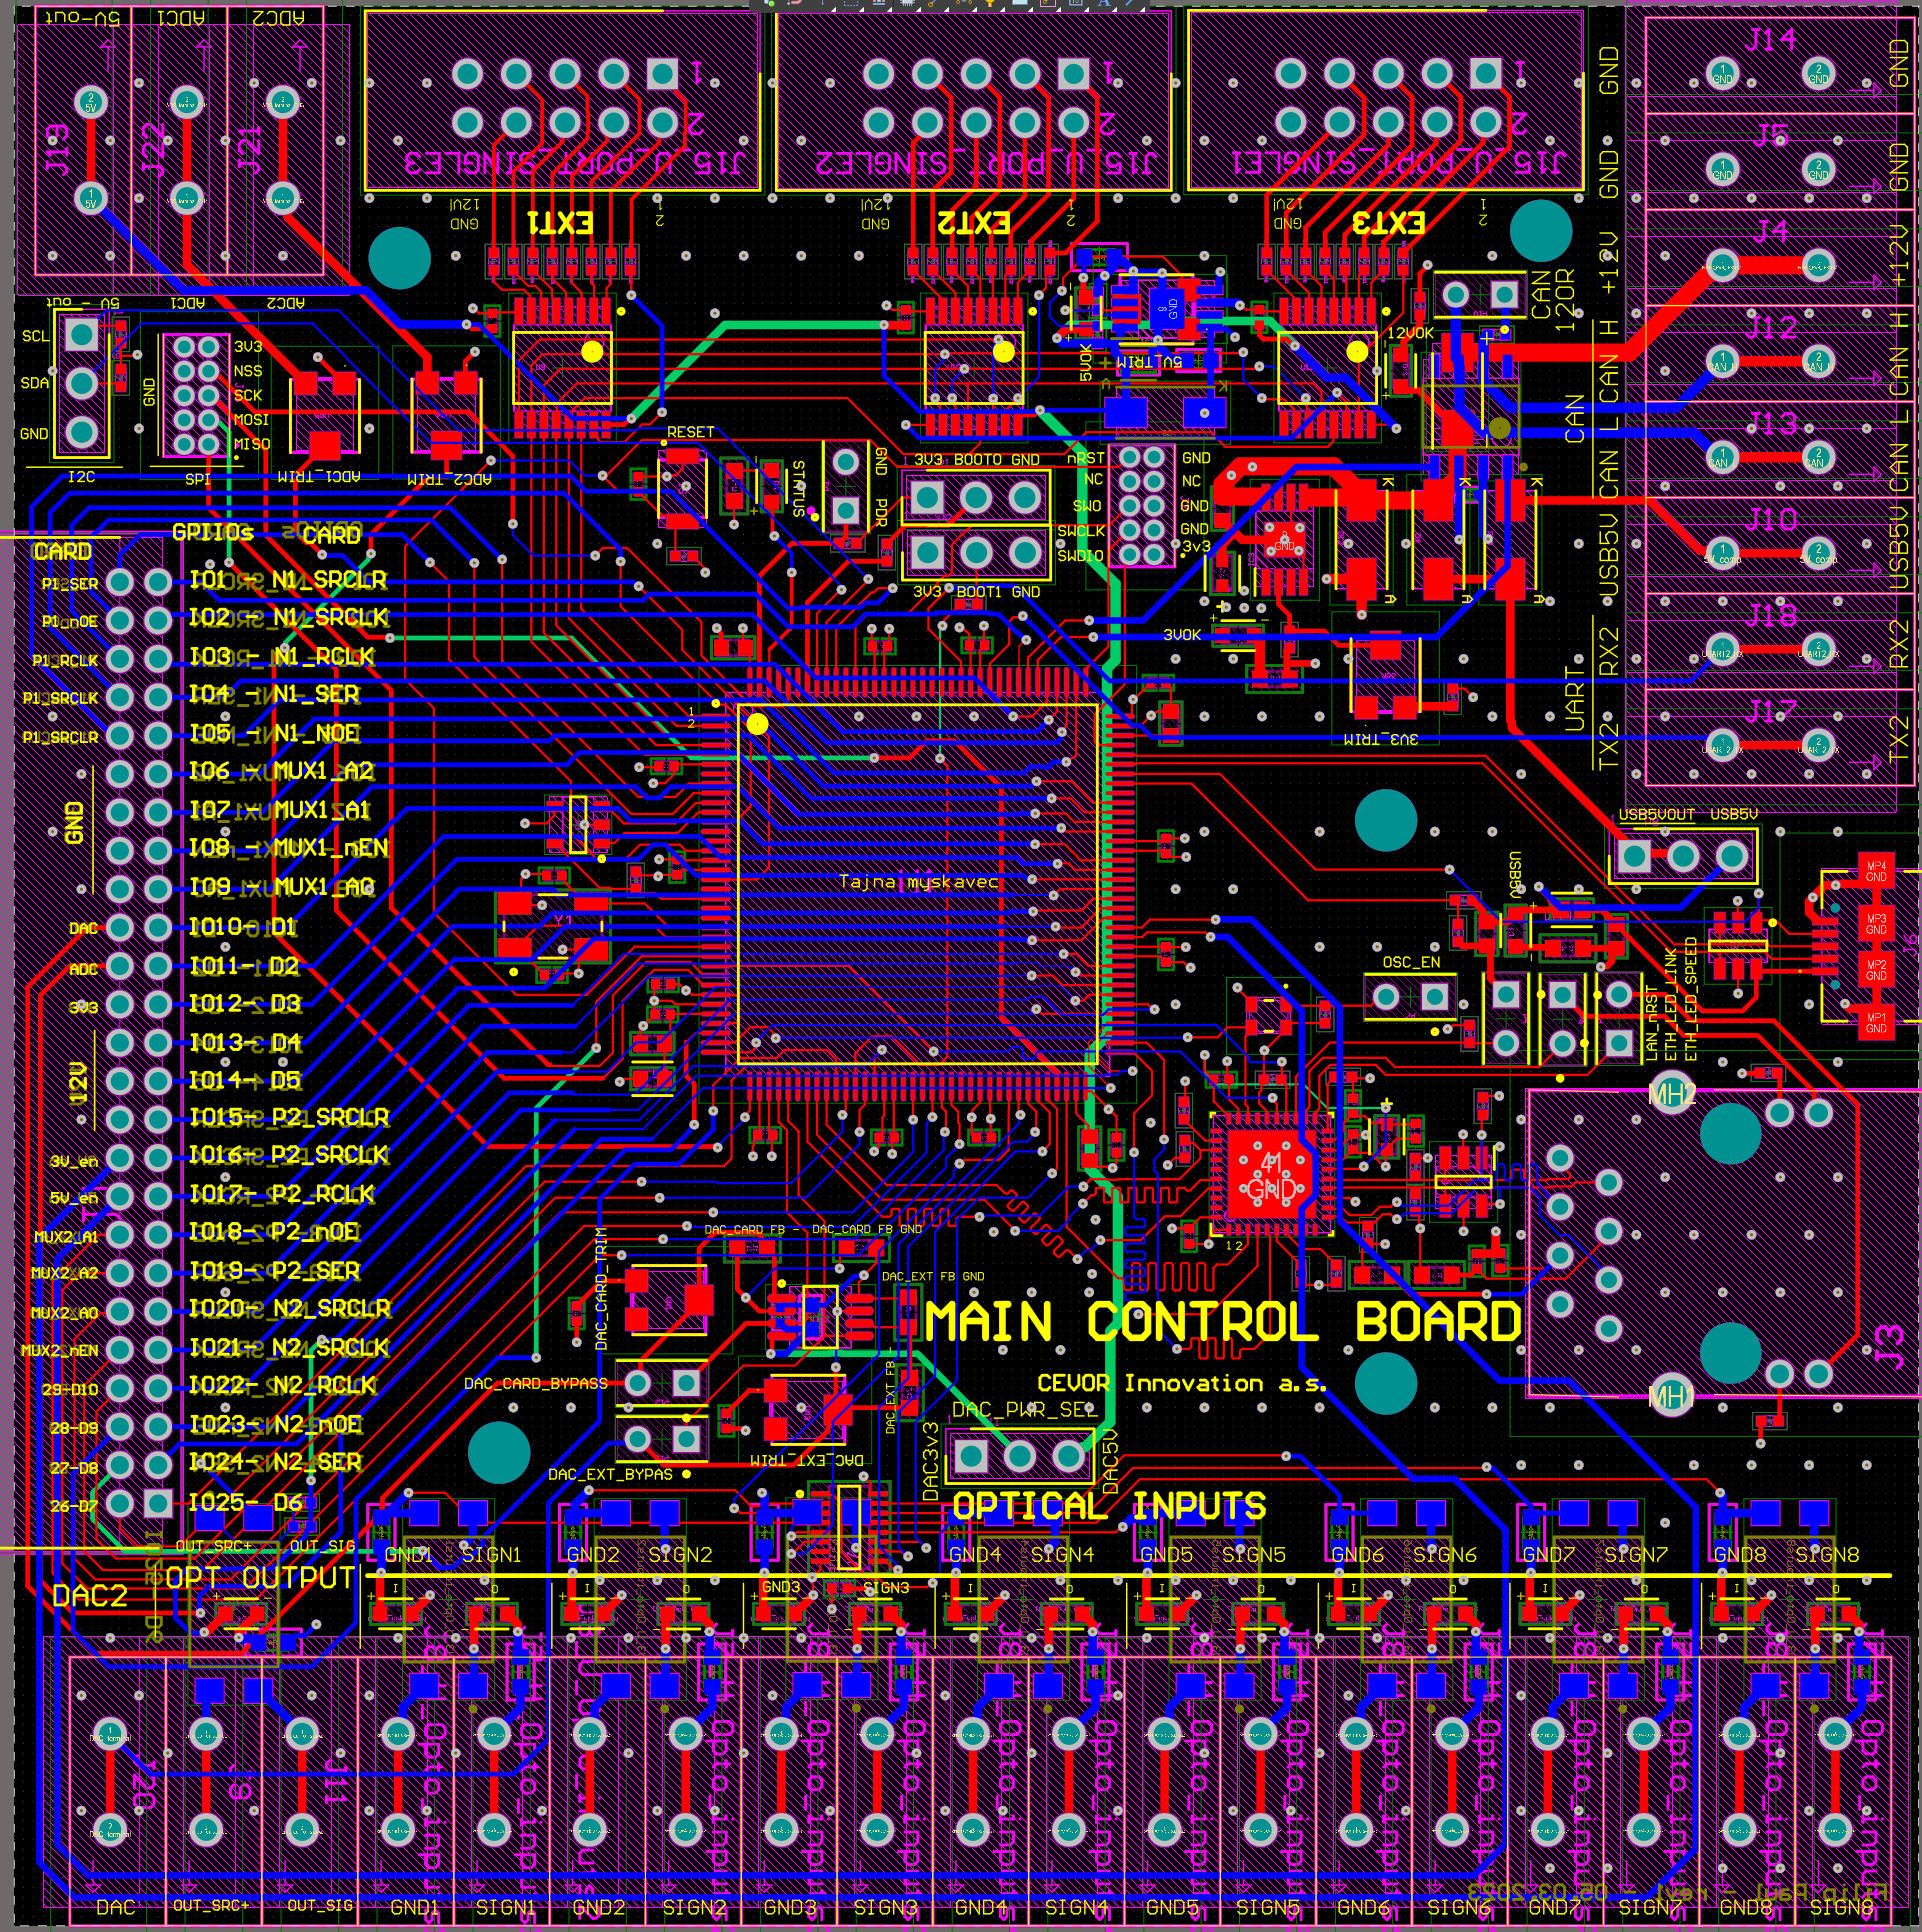
\includegraphics[width = 1\textwidth]{obrazky/all_layers_no_poly_control.png}
    \caption{Návrh PCB ovládací karty - všechny vrstvy bez polygonů}
    \label{fig:Všechny vrstvy bez polygonů control}
\end{figure}